\subsection{Problema de corte de vara}

El problema de corte de vara consiste en determinar cuál es la forma más rentable de cortar una vara de longitud \(n\), si cada posible longitud entera se vende a un precio específico (y cada corte es gratis).

Las entradas del problema son entonces la longitud de la vara \(n\in \mathbb{N}\) y un arreglo \(p\) donde \(p[i]\) es el precio de una vara de longitud \(i\):
\begin{especificacion}
  \entrada{Longitud de la vara \(n\) y arreglo \(p\) de precios.}
  \salida{Los ingresos máximos que se pueden obtener.}
\end{especificacion}
En ese modelo, \(p[0] = 0\) porque no se puede vender una longitud de \(0\).

Considérese la instancia del problema con \(n=4\) y \(p = [0, 1, 5, 8, 9]\). En ese caso:
\begin{itemize}
  \item Si no se corta la vara, se vende a \(p[4]\), o sea a \(\$9\).
  \item Si se corta en un pedazo de longitud \(3\) y otro de longitud \(1\), se venden a \(\$8\) y \(\$1\), respectivamente, para obtener ingresos de \(\$9\).
  \item Si se corta en dos pedazos de longitud \(2\), se venden a \(\$10\).
  \item Si se corta en pedazos de longitud \(2\), \(1\) y \(1\), se venden a \(\$7\).
  \item Si se corta en cuatro pedazos de longitud \(1\), se venden a \(\$4\).
\end{itemize}
Entonces, la mejor forma de cortar la vara es en dos pedazos de longitud \(2\), para obtener ingresos de \(\$10\).

\subsubsection{Combinaciones a contemplar}

Para un valor arbitrario de \(n\), hay muchas formas de cortar la vara. En cada unidad de longitud, hay dos alternativas: se corta o no. Entonces hay \(2\) posibilidades para cada una de las \(n-1\) unidades de longitud (\(n-1\) porque en la longitud \(n\) ya no se puede cortar), lo que da \[\underbrace{2\cdot2\cdots2}_{n-1 \text{ veces}} = 2^{n-1}\] combinaciones totales.

El conteo anterior no contempla que algunas combinaciones están repetidas, porque el orden de los pedazos no importa: es lo mismo cortar en la primera unidad de longitud y obtener un pedazo de longitud \(1\) y otro de longitud \(n-1\), que en la penúltima unidad de longitud. Esa observación implica que en lugar de pensar en cortar o no en cada unidad, se puede pensar en cortar de forma que los pedazos queden en tamaño no decreciente. Eso contempla todas las distintas combinaciones: aunque no contempla, por ejemplo, (\(n-2\), \(2\)), ni (\(n-2\), \(1\), \(1\)); sí contempla (\(2\), \(n-2\)) y (\(1\), \(1\), \(n-2\)), que son equivalentes. Eso reduce el número de combinaciones a la función de partición de enteros, \(\mathrm{e}^\mathrm{\pi}\sqrt{2n/3}/(4n\sqrt{3})\) (un resultado poco trivial de alcanzar), que igual sigue lejos de ser polinomial.

\subsubsection{Propiedades}

Para pensar en si el problema presenta subestructura óptima, considérese una vara de longitud \(n\). Supóngase que para venderla al mejor precio, en algún momento toca cortar en la longitud \(k\). Eso modela todos los posibles escenarios, incluso en el que lo óptimo es no cortar (\(k = n\)).

Al realizar el corte se obtienen dos segmentos de tamaños \(k\) y \(n-k\). Como \(k\) es un corte necesario para la solución óptima, entonces los tamaños \(k\) y \(n-k\) tienen que poderse cortar de forma que se vendan al mejor precio. Si no, cortar en \(k\) no produciría el mejor precio.

Ese raciocinio lleva a la subestructura óptima del problema: las soluciones óptimas a los subproblemas, en este caso la mejor forma de cortar varas de longitudes \(k\) y \(n-k\), ayuda obtener una solución óptima para el problema, que en este caso contiene un corte en \(k\).

En cuanto a problemas superpuestos, es más fácil de ver. Para % TODO!

\subsubsection{Modelo}

El estado es lo que cambia el subproblema. En este caso, es claro que una longitud distinta de vara da un subproblema diferente. 
Por qué no la tabla de precios.

Para diseñar una relación de recurrencia:
\begin{itemize}
  \item El primer caso de cortar en la primera unidad de longitud. Eso arroja un pedazo de longitud \(1\) y otro de longitud \(n-1\). Ese último pedazo de longitud \(n-1\) se puede seguir cortando (si \(n\) es grande) y entonces se tiene el mismo problema: cuál es la forma de cortarlo para maximizar los ingresos.
  \item El segundo caso es cortar en la segunda unidad de longitud y es análogo: el pedazo de longitud \(2\) se vende a \(p[2]\), pero falta evaluar cómo cortar el pedazo de longitud \(n-2\) de forma óptima.
\end{itemize}

Generalizando esos dos casos a un corte en la iésima unidad de longitud, se obtiene la relación de recurrencia para \(r(n)\), el mejor ingreso posible al cortar una vara de longitud \(n\):
\[
r(n) = \begin{cases}
  0 & \text{si } n = 0. \\
  \displaystyle\max_{1 \le i \le n} \big( p[i] + r(n-i) \big) & \text{si } n > 0.
\end{cases}
\]

En cuanto al grafo de dependencias, dado que \(r(n)\) contempla cortar en cualquier unidad de longitud de \(1\) a \(n\), el estado \(n\) depende de las soluciones a \emph{todos} los subproblemas de longitud menor: \(r(0), r(1), \ldots, r(n-1)\). Eso aplica para cualquier estado \(m\), no solo para \(n\): depende de \(r(0), \ldots, r(m-1)\). El único caso base es \(r(0)\), que no tiene predecesores. Por ejemplo, para los estados hasta \(n=4\) se trazan los arcos \(0 \to 1\); \(0 \to 2\) y \(1 \to 2\); \(0 \to 3\), \(1 \to 3\) y \(2 \to 3\); y \(0 \to 4\), \(1 \to 4\), \(2 \to 4\) y \(3 \to 4\):

\begin{center}
\setbox0=\hbox{%
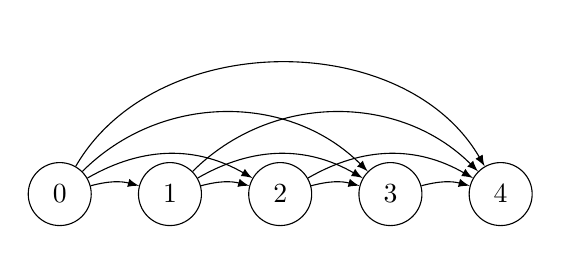
\begin{tikzpicture}[
  vertex/.style={circle, draw, minimum size=0.8cm, inner sep=0pt},
  -latex,
]
  \foreach \i in {0,...,4} {
    \node[vertex] (v\i) at (1.4*\i, 0) {\i};
  }

  \draw (v0) to[bend left=15] (v1);

  \draw (v0) to[bend left=30] (v2);
  \draw (v1) to[bend left=15] (v2);

  \draw (v0) to[bend left=45] (v3);
  \draw (v1) to[bend left=30] (v3);
  \draw (v2) to[bend left=15] (v3);

  \draw (v0) to[bend left=60] (v4);
  \draw (v1) to[bend left=45] (v4);
  \draw (v2) to[bend left=30] (v4);
  \draw (v3) to[bend left=15] (v4);
\end{tikzpicture}%
}
\ifdim\wd0>\textwidth
  \resizebox{\textwidth}{!}{\copy0}
\else
  \makebox[\linewidth]{\copy0}
\fi
\captionof{figure}{Grafo de dependencias de \(r(n)\) para \(n=4\).}
\label{fig:corte_vara_grafo_dependencias}
\end{center}

\subsubsection{Solución recursiva}
\label{sec:corte_vara_recursiva}

Para diseñar una solución recursiva, lo primero que hay que pensar es cómo dividir este problema en subproblemas. En este caso es relativamente fácil, porque dada una vara de longitud \(n\), se querría evaluar:

Con eso es fácil construir una implementación recursiva, \inline{rod_cut_rec} que evalúe el primer caso como \inline{p[1] + rod_cut_rec(n-1, p)}; el segundo, como \inline{p[2] + rod_cut_rec(n-2, p)} y así hasta \inline{p[n] + rod_cut_rec(0, p)}, donde ese último llamado recursivo evidentemente es un caso base.
\begin{codeblock}[Corte de vara recursivo.][impl:rod_cut_recursivo]
\begin{pseudocode}
def rod_cut_rec(n: int, prices: arreglo[int]) -> int:
    if n == 0: return 0

    optimal_rev = |\(-\infty\)|
    for i=1 to n:
        optimal_rev = max(optimal_rev, prices[i] + rod_cut_rec(n-i, prices))

    return optimal_rev
\end{pseudocode}
\end{codeblock}

\subsubsection{Solución top-down}
\label{sec:corte_vara_top_down}

Para eliminar la redundancia que introducen los problemas superpuestos, se implementa un algoritmo top-down. Se añade una función principal que crea un arreglo donde la función auxiliar recursiva memoiza el cálculo del mejor precio para cada longitud.
\begin{codeblock}[Corte de vara top-down.][impl:rod_cut_top_down]
\begin{pseudocode}
def rod_cut_top_down(n: int, prices: arreglo[int]) -> int:
    |\br{arri}|optimal_revs = |\textrm{arreglo de }|int|\textrm{ de longitud \(n+1\)}|
    optimal_revs[0] = 0
    for i=1 to n:
        optimal_revs[i] = |\(-\infty\)||\br{arrf}|

    return rod_cut_memo(n, prices, optimal_revs)

def rod_cut_memo(n: int, prices: arreglo[int], optimal_revs: arreglo[int]) -> int:
    |\br{memoi}|if optimal_revs[n] >= 0:
        return optimal_revs[n]|\br{memof}|

    optimal_rev = |\(-\infty\)|
    for i=1 to n:
        optimal_rev = max(optimal_rev, prices[i] + rod_cut_memo(n - i, prices, optimal_revs))

    |\br{reti}|optimal_revs[n] = optimal_rev
    return optimal_rev|\br{retf}|
\end{pseudocode}
\begin{annotations}
  \codebrace[xshift=4cm, width=6.5cm]{arri}{arrf}{Se crea el arreglo lleno de \(-\infty\) (salvo el caso base) para indicar las soluciones que aún no se han memoizado.}
  \codebrace[width=8cm]{memoi}{memof}{Si el valor está memoizado, se retorna enseguida para no recomputarlo.}
  \codebrace[xshift=2.5cm, width=5cm]{reti}{retf}{Justo antes de retornar el valor, se memoiza para los llamados siguientes.}
\end{annotations}
\end{codeblock}

\subsubsection{Solución bottom-up}
\label{sec:corte_vara_bottom_up}

Para diseñar el algoritmo bottom-up se debe reemplazar la recursión del algoritmo top-down por un ciclo. 

En el algoritmo top-down, los llamados recursivos a la función auxiliar \inline{rod_cut_memo}, con distintos valores como argumento para \inline{n}, representan los subproblemas: cada llamado evalúa cómo cortar una posible longitud de la vara (dada por un valor distinto de \inline{n}).

Como en la solución bottom-up no se invocan funciones auxiliares, el valor de \inline{n} que entra como parámetro no cambia. Por tanto, el ciclo que hace falta introducir, que reemplaza la recursión, es uno que revisa todos los posibles valores de \inline{n}, es decir todos los subproblemas, y para cada uno de ellos sigue la misma lógica que la función auxiliar de la versión top-down. Con eso, la solución bottom-up acaba con dos ciclos: uno externo, que toma el lugar de la recursión, y uno interno, idéntico al ciclo único de los algoritmos previos.

\begin{codeblock}[Corte de vara bottom-up.][impl:rod_cut_bottom_up]
\begin{pseudocode}
def rod_cut_bottom_up(n: int, prices: arreglo[int]) -> int:
    |\br{arri}|optimal_revs = |\textrm{arreglo de }|int|\textrm{ de longitud \(n+1\)}|
    optimal_revs[0] = 0|\br{arrf}|

    |\bxl{cic}|for subprob_len=1 to n:|\bxr{cic}|
        optimal_rev = |\(-\infty\)|
        |\br{inti}|for i=1 to subprob_len:
            optimal_rev = max(optimal_rev, prices[i] + optimal_revs[subprob_len-i])|\br{intf}|

        optimal_revs[subprob_len] = optimal_rev
    
    return optimal_revs[n]
\end{pseudocode}
\begin{annotations}
  \codebrace[xshift=5cm, width=7cm]{arri}{arrf}{Como el arreglo se llenará en orden, no hay que llenarlo de antemano como en top-down, con el primer elemento basta.}
  \codenote[xshift=0.5cm, width=10.5cm]{cic}{En top-down, la longitud \inline{n} cambia en cada llamado recursivo para cada subproblema; acá, \inline{n} nunca cambia, entonces \inline{subprob_len} toma su rol como la longitud de cada subproblema.}
  \codebrace[xshift=4.5cm, width=5cm, yshift=-0.2cm]{inti}{intf}{El ciclo interno es calcado de las versiones anteriores, pero la tabulación reemplaza la recursión.}
\end{annotations}
\end{codeblock}

Esa solución cuenta con complejidad temporal de \(\Theta(n^2)\), por los dos ciclos anidados, y con complejidad espacial de \(\Theta(n)\), por el arreglo que se utiliza para la tabulación.

\subsubsection{Obtener los tamaños de los cortes}

Inicialmente, el problema de corte de vara se planteó como un problema de optimización, donde la respuesta esperada era el máximo ingreso posible. Sin embargo, el problema se podría plantear como un problema de búsqueda en el que se busca alguna configuración de cortes que maximiza el ingreso, en lugar del ingreso en sí.
\begin{especificacion}
  \entrada[Entradas]{Un entero \(n\) que representa la longitud de la vara y un arreglo \(p\) de tamaño \(n+1\), donde \(p[i]\) es el precio de una vara de longitud \(i\).}
  \salida{Una pila con las longitudes de las piezas que maximizan el precio de venta.}
\end{especificacion}

Para esto, al implementar el algoritmo de programación dinámica se debe no solo computar el valor óptimo sino también almacenar información para que, una vez se obtenga el valor óptimo, se pueda recuperar los pasos que se siguieron para obtenerlo. 

En este caso, además de almacenar el precio óptimo para una longitud \(\ell\), se almacena el primer corte que corresponde a ese precio óptimo. Solo se almacena el primer corte \(c\) para cada longitud, porque para determinar posteriormente el resto de cortes (si se requieren más de un corte), basta con examinar el subproblema de la longitud restante, o sea, el subproblema de la vara de longitud \(\ell-c\) (para el cual también se guardó el primer corte).

\begin{codeblock}[Corte de vara con reconstrucción de cortes.][impl:rod_cut_reconstruccion]
\begin{pseudocode}
def rod_cut(n: int, prices: arreglo[int]) -> pila[int]:
    optimal_revs = |\textrm{arreglo de }|int|\textrm{ de longitud \(n+1\)}|
    optimal_revs[0] = 0
    optimal_cuts = |\textrm{arreglo de }|int|\textrm{ de longitud \(n+1\)}|

    for subprob_len=1 to n:
        optimal_rev = |\(-\infty\)|
        for i=1 to subprob_len:
            revenue = prices[i] + optimal_revs[subprob_len-i]
            if revenue > optimal_rev:
                optimal_rev = revenue
                |\bxl{mejor}|optimal_cut = i|\bxr{mejor}|
        optimal_revs[subprob_len] = optimal_rev
        |\bxl{optm}|optimal_cuts[subprob_len] = optimal_cut|\bxr{optm}|

    segments = |\textrm{pila de }|int|\textrm{ de longitud máxima \(n\)}|
    |\br{cortsi}|i = n
    while i > 0:
        cut = optimal_cuts[i]
        segments.put(cut)
        i -= cut|\br{cortsf}|

    return segments
\end{pseudocode}
\begin{annotations}
    \codenote[notepos={(cn@mejor.east)+(5cm,0.6cm)}, curve={bend right=5}, width=4.7cm]{mejor}{Se almacena el primer corte que se hizo en la solución óptima de ese subproblema.}
    \codenote[xshift=1.5cm, width=6.3cm]{optm}{Para una longitud \(\ell\), el primer corte es \inline{cortes_optimos[\(\ell\)]}; los cortes restantes (si hay) se deben averiguar mirando el subproblema de la longitud restante, que es \inline{\(\ell - \)cortes_optimos[\(\ell\)]}}
    \codebrace[xshift=2.5cm, width=8.5cm]{cortsi}{cortsf}{Se toma el primer corte óptimo para \inline{n}; se resta de \inline{n} para obtener una nueva longitud, luego se mira el primer corte para ella; y así hasta acabar la vara}
\end{annotations}
\end{codeblock}

\practicar[gfg]{Rod Cutting}{https://www.geeksforgeeks.org/problems/rod-cutting0840/1}
